\chapter{保障项目进度}
\section{项目进度管理的概述}
\subsection{项目进度管理的重要性}
进度问题是项目生命周期内造成项目冲突的主要原因。
时间易于测量、易于成为焦点。
\subsection{项目进度及项目进度管理}
项目进度是执行项目各项活动和到达里程碑的计划日期。
\par 进度管理是采用科学的方法确定进度目标,编制进度计划和资源供应计划,进行进度控制,在与质量、费用目标协调的基础上,实现工期目标。
\subsection{项目进度管理过程}
\begin{enumerate}
	\item 活动定义:确定完成项目可交付成果而需开展的具体活动。
	\item 活动排序:识别和记录计划活动之间相互逻辑关系的过程。
	\item 活动资源估算:估算完成计划活动所需资源类型和数量。
	\item 活动持续时间估算:估算完成单项计划活动的时间。
	\item 进度计划编制:分析计划活动顺序、计划活动持续时间、资源要求和进度制约因素,制定项目进度表。
	\item 进度控制:对项目进度变更进行控制,确保项目目标的实现。
\end{enumerate}
\begin{figure}[!h]
	\centering
	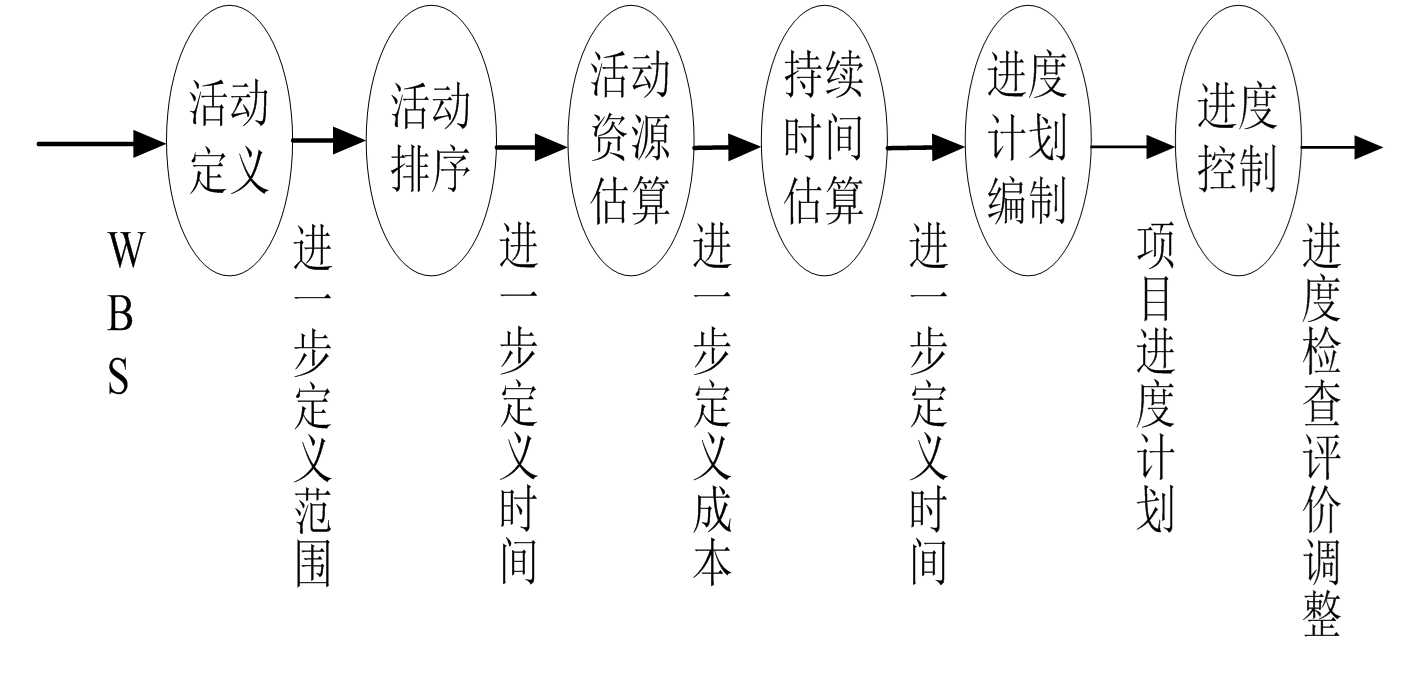
\includegraphics[width=0.8\textwidth]{image/5-1}
	\caption{项目时间管理过程}
\end{figure}
\section{活动定义}
项目活动定义是为了保障项目目标实现而开展的对已确认的项目工作包的进一步分解和界定,并从中识别出为生成项目产出物所必需的各种项目活动。 
\par 定义的主要依据主要有:WBS、项目范围说明书、组织的过程资产和项目管理计划等。时间管理最初3个过程的基本顺序:
\begin{itemize}
	\item 活动定义(进一步定义范围)
	\item 活动排序(进一步定义时间) 
	\item 活动资源估计(进一步定义成本)
\end{itemize}
\subsection{进一步分解项目工作}
\begin{itemize}
	\item 应该将项目工作分解为更小、更易管理的活动或任务;
	\item 这些小的活动应该是能够保障完成交付产品项目的可实施的详细任务,而不是指可交付物。
	\item 要将所有活动列成一个明确的活动清单,让每一个成员能够清楚有多少工作需要处理。
\end{itemize}
\subsection{项目活动特征}
\begin{enumerate}
	\item 对于需要执行的活动,应以动词或形容词加名词方式描述。
	\item 如果一个资源分配给一项活动,应该由一个人管理交付。
	\item 每一项活动要定义好一个开始点。
	\item 一项活动存在一个有形的输出或完成的产品。
	\item 活动在逻辑上应与WBS元素相符。
	\item 对于每一项活动要有充足的控制量和时间。
	\item 开始和结束点必须充分定义,并能汇报活动的开始和完成。
	\item 从活动或包含活动的工作包中能够计算出实际成本。
	\item 活动反映了除细微或偶发的活动外的项目目标的重要工作。
	\item \underline{零持续时间活动是里程碑或事件},代表了另一项活动或一组活动的开始或完成。
\end{enumerate}
\subsection{项目活动定义的结果}
项目活动定义的结果:项目活动清单、相关支持信息、活动属性、更新的WBS、里程碑清单。
\section{活动排序}
\subsection{活动排序的依据}
主要依据有:
\begin{itemize}
	\item 项目活动清单及相关支持信息
	\item 项目范围说明书
	\item 里程碑清单
	\item 排序应确定的各种关系、限制和假设
\end{itemize}
\subsection{前导图法与箭线图法}
项目网络图是项目活动之间的逻辑关系或排序的图形显示,如前导图法与箭线图法 。
\subsubsection{前导图法(PDM)}
前导图法是一种用节点表示活动、箭线表示活动关系的项目网络图。
\begin{itemize}
	\item 在这种方法中,每项活动有惟一的活动号,每项活动都注明了预计的工期;
	\item 每个节点的活动会有如下几个时间:最早开始时间、最迟开始时间、最早结束时间和最迟结束时间;
	\item 在前导图中,箭尾节点表示的活动是箭头节点的紧前活动;箭头节点表示的活动是箭尾节点的紧后活动。
\end{itemize}
\begin{figure}[!h]
	\centering
	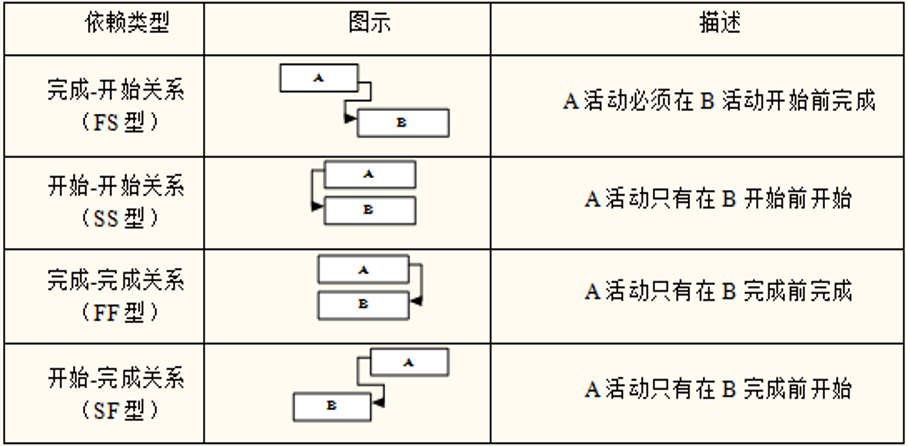
\includegraphics[width=0.8\textwidth]{image/5-2}
	\caption{前导图法中活动之间的四种依赖关系}
\end{figure}
绘制前导图时,需要遵守下列规则:
\begin{enumerate}
	\item 前导图必须正确表达项目中活动之间的逻辑关系。
	\item 在图中不能够出现循环回路。
	\item 在图中不能出现双向箭头或无箭头的连线。
	\item 图中不能出现无箭尾节点的箭线或无箭头节点的箭线。
	\item 图中只能有一个起始节点和一个终止节点。 
\end{enumerate}
\begin{figure}[!h]
	\centering
	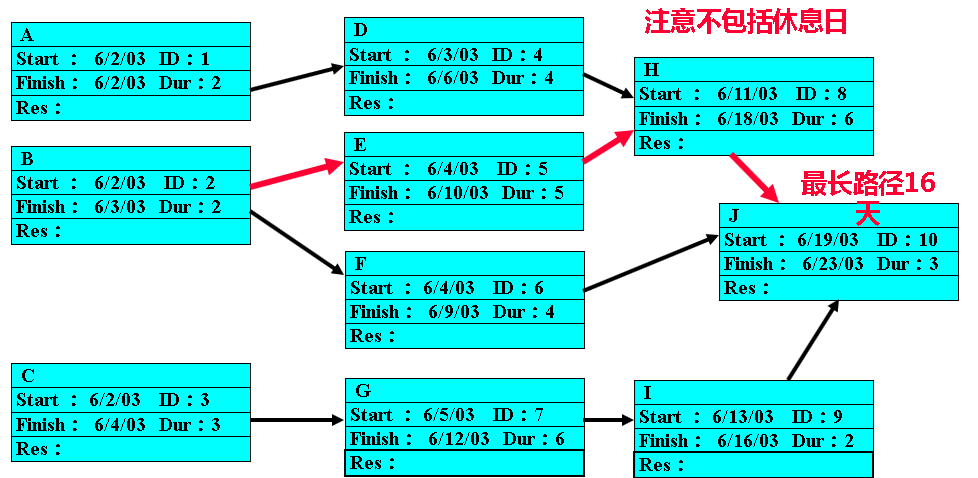
\includegraphics[width=\textwidth]{image/5-3}
	\caption{采用 PDM 绘制的项目网络图示例}
\end{figure}
\subsubsection{箭线图法(ADM)}
ADM法与PDM法的表示方法相反,它是一种用箭线表示活动、节点表示活动排序的网络图方法。
\begin{itemize}
	\item 一项活动都用一根箭线和两个节点来表示,每个节点有个号码,箭线的箭尾节点和箭头节点是该项活动的起点和终点。
	\item 依据是否需消耗时间或资源,可将活动分为实活动或虚活动。
\end{itemize}
\begin{figure}[!h]
	\centering
	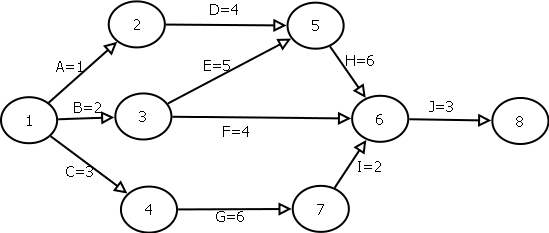
\includegraphics[width=0.8\textwidth]{image/5-4}
	\caption{采用ADM绘制的项目网络图示例}
\end{figure}
\section{活动资源和活动持续时间估算}
\subsection{活动资源估算}
活动资源估算包括决定需要什么资源和每一种资源应该需要多少,以及何时使用资源来有效地执行项目活动。
\par 估算方法:专家判断法、多方案分析法、自上而下的估算方法、使用估算软件。
\par 活动资源估算过程的输出是识别和说明工作包中的每一个计划活动所需要的资源类型和数量,这些资源汇总决定了每个工作包所需要的资源。 
\subsection{活动持续时间估算}
活动持续时间估算是项目制定计划的一项重要工作,它直接关系到各事项、各工作网络时间的计算和完成整个项目任务所需要的总时间。
\begin{figure}[!h]
	\centering
	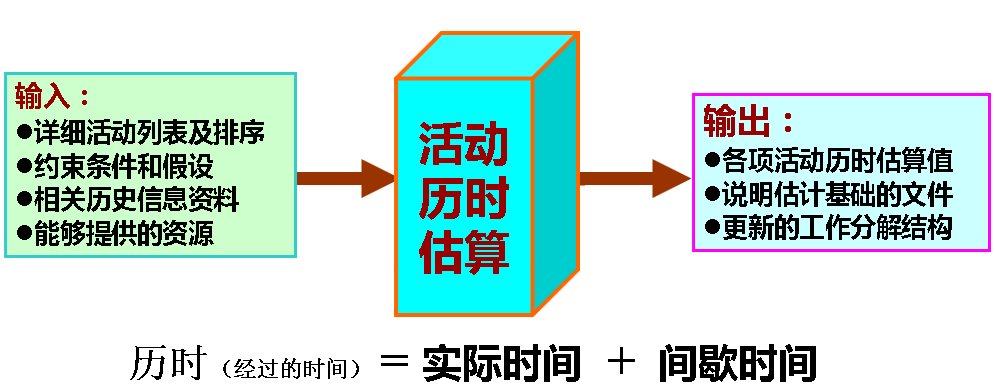
\includegraphics[width=\textwidth]{image/5-5}
	\caption{活动持续时间估算}
\end{figure}
\section{编制项目进度计划}
\textbf{制定进度计划的目标:}建立一个现实的项目进度计划,为监控项目的时间进展情况提供一个基础。
\par 制定进度计划的方法:应用定义、排序、估算等过程得到的结果,制定进度计划,决定项目的开始日期和完成日期。
\subsection{进度计划的内容}
进度计划的内容:项目综合进度计划、项目实施进度计划、项目采购进度计划、项目验收进度计划、项目维护计划。
\subsection{编制进度计划的依据}
进度计划的编制,是建立在项目目标、资源、经验和各种约束条件的基础上的,其主要依据有:项目网络图、项目活动持续时间估算、项目活动资源估算、资源的可用性、约束条件、风险记录、项目团队的作息制度与政策因素。
\subsection{编制进度计划的方法}
\subsubsection{关键路径法 (Critical Path method)}
关键路径法(CPM),也称为关键路径分析,是预测总体项目历时的网络分析技术,是帮助人们分析与解决进度拖延的一种重要工具。
\par 一个项目的关键路径是指一系列决定项目最早完成时间的活动。它是项目网络图中最长的路径,并且有最少的浮动时间或时差。
\par 利用关键路径分析平衡进度计划 、缩短关键路径上的活动历时、关注与及时更新关键路径数据。\\
\newline
\fbox{
	\parbox{\textwidth}{
		\begin{itemize}
			\item $\text{最早开始时间}ES=max\{\text{紧前活动的EF}\}$
			\item 最早完成事件$EF=ES+D$
			\item 最迟完成时间$LF=min\{\text{紧后活动的}LS\}$
			\item 最迟开始时间$LS=LF-D$
			\item 时差
			\subitem $\text{总时差}TF=LS-ES$
			\subitem $\text{自由时差}FF=min\{\text{紧后活动的}ES\}-EF$
			\item 关键路径:网络图中最长路径;
		\end{itemize}
	}
}
\newline\\
例题:假设活动A的最早开始时间为0,活动M的最迟完成时间为47。仔细分析该项目图示后回答如下问题:
\begin{figure}[!h]
	\centering
	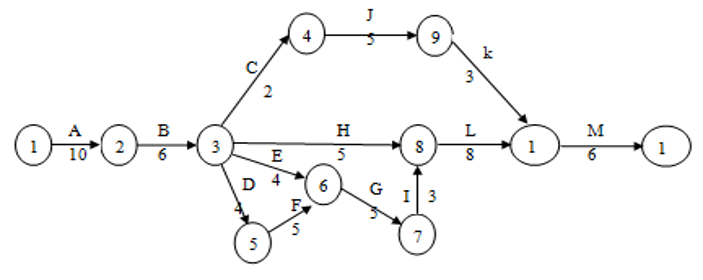
\includegraphics[width=0.8\textwidth]{image/5-6}
	\caption{关键路径分析例子}
\end{figure}
\begin{itemize}
	\item 计算活动B的最早开始时间ES(B)、最早完成时间EF(B);
	\item 计算活动G的最早开始时间ES(G)、最早完成时间EF(G);
	\item 计算活动H的最早开始时间ES(H)、最早完成时间EF(H)。
	\item 计算活动A的最迟开始时间LS(A)、最迟完成时间LF(A);
	\item 计算活动G的最迟开始时间LS(G)、最迟完成时间LF(G);
	\item 计算活动H的最迟开始时间LS(H)、最迟完成时间LF(H)。
	\item 确定该项目的关键路径、关键活动。
\end{itemize}
解:
\\最早开始时间ES、最早完成时间EF
\par $B: ES_B=10,\quad EF_B=ES_B+16=16$
\par $H: ES_H=10+6=16,\quad EF_H=ES_H+5=21$
\par $G: ES_G=max\{EF_E,EF_F\}=25,\qquad EF_G=ES_G+5=30$
\par $E:ES_E=10+6=16,\quad EF_E=ES_E+4=20$
\par $F:ES_F=10+6+4=20,\quad EF_F=ES_F+5=25$
\\最迟开始时间LS、最迟完成时间LF(先计算最后一项)
\par $B:LF_B=min\{LS_C,LS_H,LS_E,LS_D\}$
\par $M:LF_M=47,\quad LS_M=LF_M-D=47-6=41$
\par $L:LF_L=LS_M=41,\quad LS_L=LF_L-D=41-8=33$
\par $I:LF_I=LS_L=33,\quad LS_I=LF_I-D=33-3=30$
\par $G:LF_G=LS_I=30,\quad LS_G=LF_G-D=25$
\par $H:LF_H=LS_L=33,\quad LS_H=LF_H-D=33-5=28$
\par $LS_C=31,\quad LS_E=21,\quad LS_D=16$
\par $B:LF_B=min\{31,28,21,16\}=16,\quad LS_B-D=16-6=10 $
\\总时差TF和自由时差FF
\par $ES_C=16,\quad ES_E=16,\quad ES_D=16,\quad ES_I=30,\quad ES_L=33$
\par $B:TF_B=LS_B-ES_B=10-10=0$
\par $FF_B=min\{ES_C,ES_H,ES_E,ES_D\}-EF_B=0$
\newline
\par $G:TF_G=LS_G-ES_G=25-25=0$
\par $FF_G=ES_I-EF_G=30-30=0$
\newline
\par $H:TF_H=LS_H-ES_H=28-16=12$
\par $FF_H=ES_L-EF_H=33-21=12$
\\关键路径和关键活动
\par $A\rightarrow B\rightarrow C\rightarrow J\rightarrow K\rightarrow M:32$
\par $A\rightarrow B\rightarrow H\rightarrow L\rightarrow M:35$
\par $A\rightarrow B\rightarrow E\rightarrow G\rightarrow I\rightarrow L\rightarrow M:42$
\par $A\rightarrow B\rightarrow D\rightarrow F\rightarrow G\rightarrow I\rightarrow L\rightarrow M:47$(最长为关键路径)
\subsubsection{计划评审技术 (Program Evaluation and Review Technique)}
项目时间管理的另一项技术是PERT,即当具体活动的估算存在很大的不确定性时,用来估算项目历时的一种网络分析技术。
\par PERT 将关键路径法应用于加权平均历时估算。它 采用概率时间估算,根据乐观的、最可能的、悲观的活动历时估计进行项目历时估算。
\begin{center}
	\Large{
		$
		PERT\text{加权平均}=\dfrac{\text{乐观时间}+4\times\text{最可能的时间}+\text{悲观时间}}{6}
		$
	}
\end{center}
\subsubsection{甘特图 (Gantt chart)}
甘特图通过日历形式列出项目活动及其相应的开始和日期,为反映项目进度信息提供了一种标准格式。
\par 甘特图的早期版本只是在左边的一栏中列出项目活动或任务、在右边的一栏中列出日历时间单位,人们形象地叫它为横道图。应该与WBS中的活动相一致。
\subsection{进度计划编制的结果}
项目进度计划至少包括每一项详细活动的计划开始日期和预期完成日期。
\par 项目进度计划可用简要的文字形式描述,也可用图表的形式给出,图表的常用表示形式为:带日期信息的项目网络图、甘特图、里程碑图和项目进度计划表。
\subsection{计划编制中的问题与对策}
计划的编制,在强调实现性、指导性和可操作性 的同时,需要注意如下问题:
\begin{itemize}
	\item 不要忽略损失的时间 
	\item 明确项目工作实施顺序和时间
	\item 明确一个适当的工期
	\item 把握计划粗细的程度
\end{itemize}
\section{项目进度控制}
项目进度控制的关键是\textbf{监控项目的实际进度,及时将它与计划进度进行比较,采取必要的措施纠正偏差。}
进度控制的内容主要包括:
\begin{itemize}
	\item 确定项目的进度是否发生变化,找出变化的原因,采取有效的措施纠正偏差;
	\item 对影响项目进度变化的因素进行控制,从而确保这些变化朝着有利于项目目标实现的方向发展。
\end{itemize}
\subsection{项目进度控制原则}
项目进度控制原则:动态原则 、系统原则 、循环原则、弹性原则 。
\subsection{影响项目进度的原因}
影响进度的因素很多,如人为因素、技术因素、资金因素、环境因素等。
\par 影响原因:低估了项目实现的条件、项目参与者的错误 、不可预见的事件的发生。
\subsection{项目进度控制的过程}
\begin{figure}[!h]
	\centering
	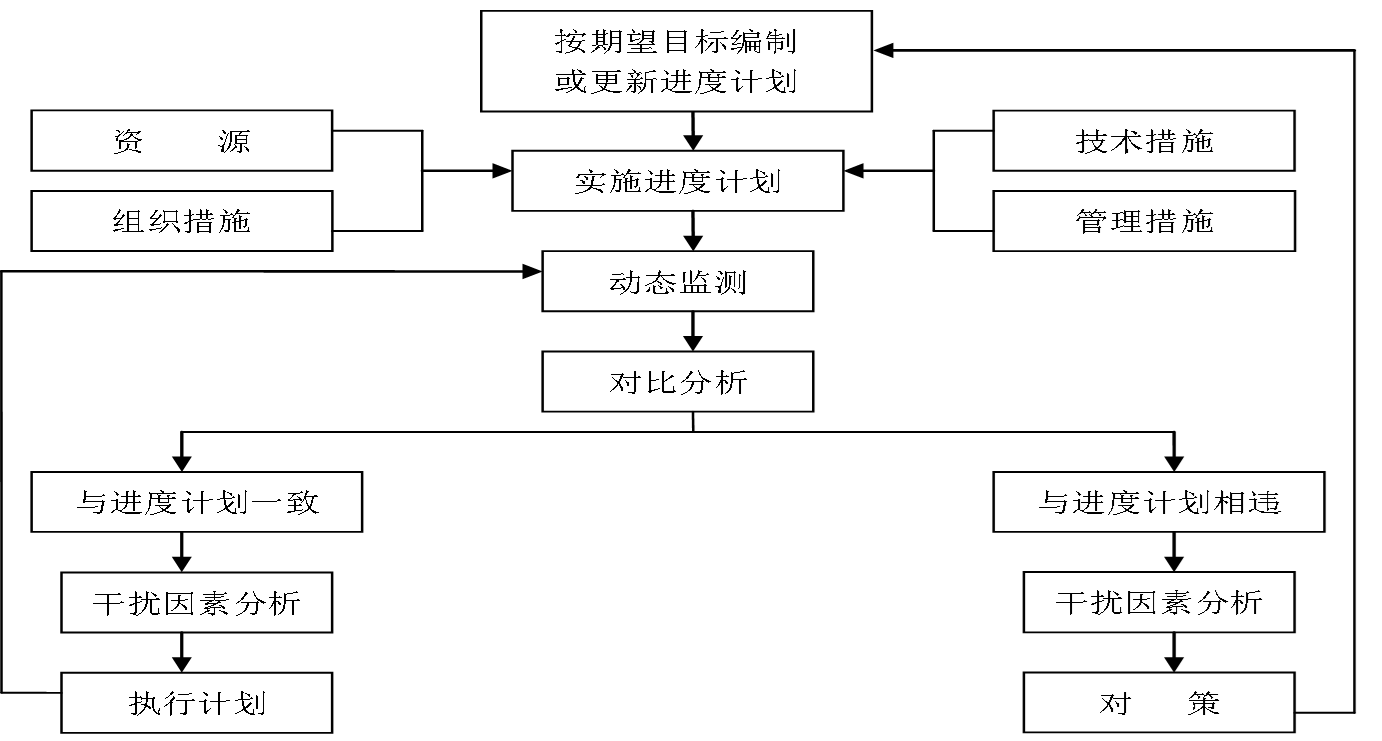
\includegraphics[width=0.8\textwidth]{image/5-7}
	\caption{项目进度控制过程图}
\end{figure}
\subsection{进度控制方法}
\begin{enumerate}
	\item 项目进度报告 :项目进度计划执行情况报告、项目详细设计检查报告、项目执行状态报告。
	\item 使用进度变更控制系统
	\item 应用项目进度管理软件 
	\item 进行比较分析 
\end{enumerate}
\subsection{IT项目进度控制}
\begin{itemize}
	\item 可用的基础:关键的干系人参与制定和一致认可项目进度计划,是计划可用的基础。
	\item 可行的基础:建立现实的项目进度计划是计划可行的基础。
	\item 可控的基础:项目经理清楚而如实地汇报项目的状态是计划可控的基础。
\end{itemize}

